\documentclass[11pt]{article}
\usepackage[top=1.00in, bottom=1.0in, left=1in, right=1in]{geometry}
\renewcommand{\baselinestretch}{1.1}
\usepackage{graphicx}
\usepackage{natbib}
\usepackage{amsmath}
\usepackage{parskip}
\usepackage{wrapfig}
\usepackage[font=small,labelfont=bf]{caption}
% counting words? https://app.uio.no/ifi/texcount/online.php

\def\labelitemi{--}
\parindent=0pt

\begin{document}
\renewcommand{\refname}{\CHead{}}
% \setlength{\parindent}{0cm}
% \setlength{\parskip}{5pt}


{\bf Title:} Strengthening forest resilience through cross-disciplinary modeling of tree growth and decline across North America 

{\bf Funding for:} 24-week fellowship for E. M. Wolkovich of UBC  (Canada)  to visit Andrew Gelman at Columbia University (USA)

\begin{abstract}
Northern hemisphere forests are critical for healthy ecosystems, healthy people and drive the economies of many countries. They are also highly threatened by multiple risks, including climate change, pests and fire. While extensive research has worked to map and model these threats, the complexity of tree growth and the multi-scale and multi-threat nature of forest health has made understanding the major drivers of forest growth and decline difficult. Here, we propose a fellowship linking the University of British Columbia (Canada) with Columbia University (USA) to bridge across disciplines (ecology, statistics and climatology) for improved models of tree and forest health. Focusing on North American forests, we will model the complexity of tree growth at the individual level then use hierarchical modeling to integrate additional effects at the species, stand and regional levels to produce a continental understanding how, where and why forests are growing or declining. We expect this project will provide major new forecasts of tree growth and forest health, that can clearly separate out the effects of individual-level tree growth from stand level properties (e.g. species mixtures) and events (e.g., fire and pest outbreaks). Such forecasts can help improve large-scale modeling of the earth system and guide managers in how to manage forests for climate resiliency. 
\end{abstract}

\setlength{\intextsep}{6pt} 
\begin{wrapfigure}{r}{0.35\textwidth}
\centering
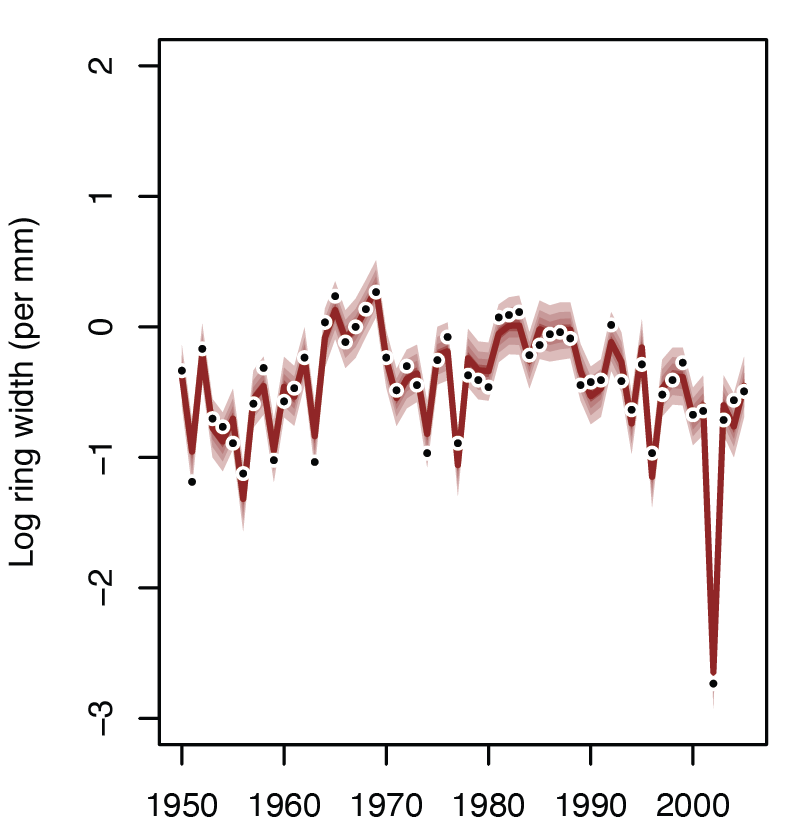
\includegraphics[width=0.33\textwidth]{figs/ut539_tree22_1panel.png}
\caption{An example of the complexity of tree growth from one \emph{Pinus ponderosa} tree sampled in Utah. Dots show the observed radial growth each year, while the coloring represents estimates from a hierarchical Gaussian process model.} 
\label{fig:onetree}
\end{wrapfigure}

The fellowship is proposed for 15 September 2027 to 29 February 2028 (24 weeks) to bring Professor Elizabeth Wolkovich to Columbia University to work with Andrew Gelman and collaborators. Wolkovich is a leading plant biology researcher who has defined and led the field of temporal ecology, focused on better understanding how biological time and climate shape plants, communities and ecosystem. Her work is highly cross-disciplinary, drawing on expertise from climatology and evolutionary biology. 

She will bring this cross-disciplinary expertise to Columbia, creating collaborations to develop better models of tree growth to strengthen and invigorate ties between the Columbia Climate School and Lamont Doherty Earth Observatory, while also building a lasting connection between UBC and Columbia. Columbia's vibrant research community across the Departments of Statistics and Political Science---where Gelman is appointed---and the University's focus on cross-disciplinary earth system science through the Columbia Climate School and Lamont is uniquely positioned to support the proposed work and make sure it is well disseminated. Gelman himself is a rare researcher who fully combines scientific and statistical approaches to solve major challenges and then communicates them broadly. While Gelman and Wolkovich have known each other through the statistical research community, they have only worked together briefly (and remotely) on a project on trophic synchrony. If funded, this fellowship would thus help launch their first major collaboration.  

The same forest types and tree species occur across Canada and the United States, making connections in forest modeling and management between these countries important, especially with continuing climate change. This project will draw on data from the International Tree Ring Data Bank (ITRDB), climate data from PRISM and NASA and new mapping efforts of fire and pest outbreaks to model tree growth across North America since 1896. Working together, Wolkovich, Gelman and colleagues will develop the exact approach during the fellowship but we expect it will build from individual-level tree models of growth with age (allometry) and in response to annual climate with additional effects at the stand (or site) and regional levels. This multi-level approach will allow us to estimate the effect of different species, different climate and events that occur at the stand-level, including fire and pest outbreaks. For climate, we plan to begin by focusing on summer warmth through growing degree days (GDD), moisture estimated through precipitation sums and stress effects possible through high vapor pressure deficit. This focus on climate will be critical for forecasting from our model to predict how forests will respond to continuing anthropogenic climate change. These forecasts will be especially unique in providing guidance on how they may shift depending on future forest species and age composition and the management of fire and pest outbreaks. % yielding a multi-risk view of our future ...

% starting with western North America!  
\end{document}
